%UNIT 2: A NUMERICAL APPROACH
%%%%%%%%%%%%%%%%%%%%%%%%%%%
%%%% Put the following at the top of each .tex file  %
\pagestyle{fancy}
\renewcommand{\theUnit}{1.4}
\ifthenelse{\isundefined{\UnitPageNumbers}}{}{\setcounter{page}{1}}
\rhead{Section \theUnit: A Numerical Approach}
\lhead{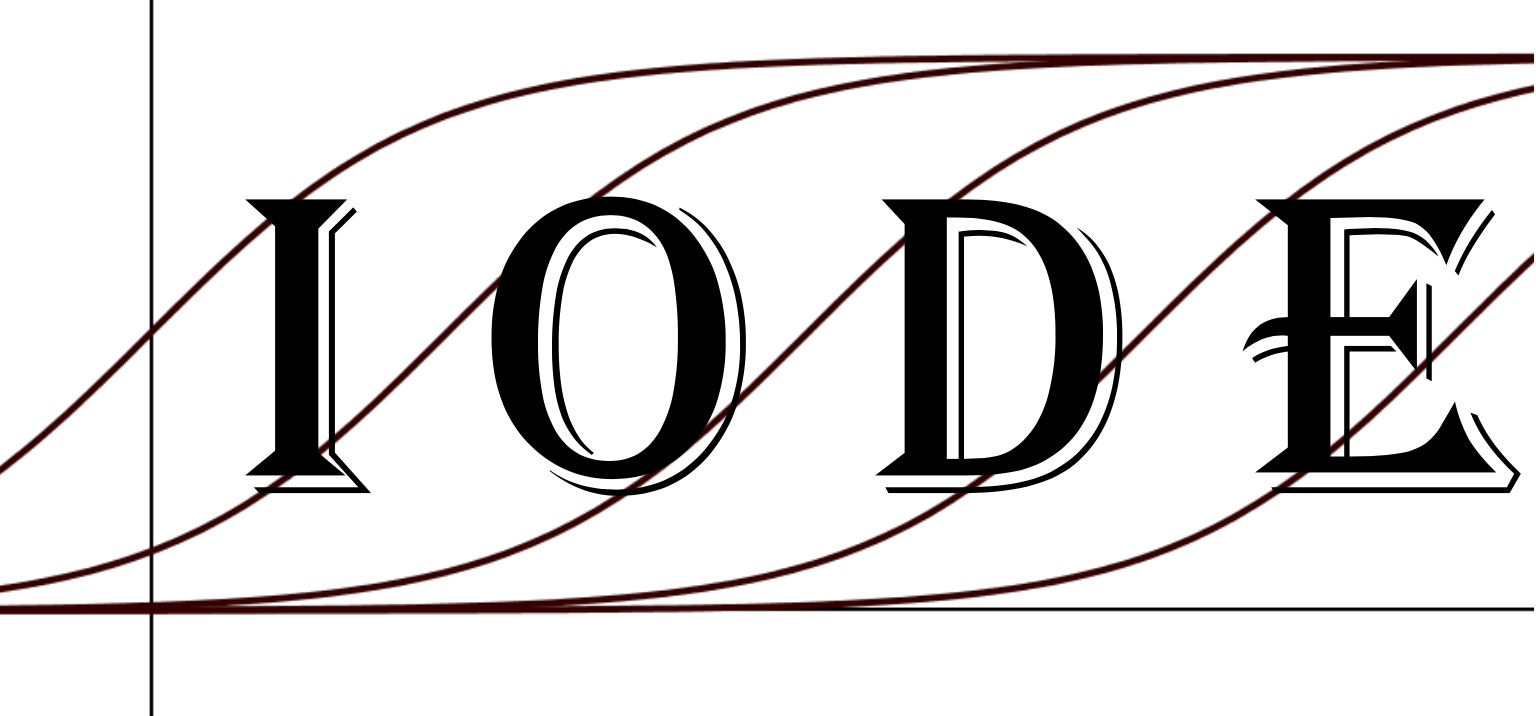
\includegraphics[width=1.25cm]{IODE-logo.png}}
\rfoot{\mypage}
\lfoot{}
\cfoot{}
\fancypagestyle{firstfooter}{\footskip = 50pt}
\renewcommand{\footrulewidth}{.4pt}
%%%%%%%%%%%%%%%%%%%%%%%%%%%
\vspace*{-20pt} \thispagestyle{firstfooter}
\pagebegin{A Rate of Change Equation for Limited Resources}

In a previous problem we saw that the rate of change equation $\displaystyle\frac{dP}{dt}=0.3P$ can be used to model a situation where there is one species, continuous reproduction, and unlimited resources. In most situations, however, the resources are not unlimited, so to improve the model one has to modify the rate of change equation $\displaystyle\frac{dP}{dt}=0.3P$ to account for the fact that resources are limited. 
\begin{enumerate}
\item	\label{02problem1}
\begin{enumerate}
\item In what ways does the modified rate of change equation \label{03problem1parta}
\[ \frac{dP}{dt}=0.3P\left(1-\frac{P}{10}\right) \] account for limited resources? (Think of 10 as scaled to mean 10,000 or 100,000) 
\vfill
\item	How do you interpret the solution with initial condition $P(0) = 10$? \label{03problem1partb}
\vfill
\item	Open the Slope Field Viewer, \href{https://ggbm.at/ZGeeGQbp}{\underline{https://ggbm.at/ZGeeGQbp}},
and plot the slope field for \[ \frac{dP}{dt}=0.3P\left(1-\frac{P}{10}\right). \]
(Note: In the Slope Field Viewer you will need to use the variable $y$ instead of $P$, and you may want to change the viewing window using the button on the right of the applet.) In what ways are your responses to parts \ref{03problem1parta} and \ref{03problem1partb} visible in the slope field? \label{03problem1partc}

\vspace{-1in}\hspace{-0.75in}
\includegraphics[width=0.5in]{03/03SlopeFieldViewerQR.png}
\vfill

\item	In this problem, negative $P$ values do not make sense, but we can still mathematically make sense of the slope field for negative $P$ values. Explain why the slope field looks the way it does below the $t$-axis. \label{03problem1partd}
\vfill
\end{enumerate}

\item If there are initially $P(0)=2$ fish in the lake, approximately how many fish are in the lake at time $t=2$?  How did you arrive at your approximation? (Hint: Initially $\frac{dP}{dt} = 0.48$, but what meaning does $0.48$ have?) \label{03problem3}
\vfill
\end{enumerate}

\clearpage
%%%%%%%%%%%%%%%%%%%%%%%%%%%%%%%%%%%
\pagebegin{Using a Slope Field to Predict Future Fish Populations}

Below is a slope field for the rate of change equation $\displaystyle \frac{dP}{dt}=0.3P\left(1-\frac{P}{10}\right).$ 
\begin{center}
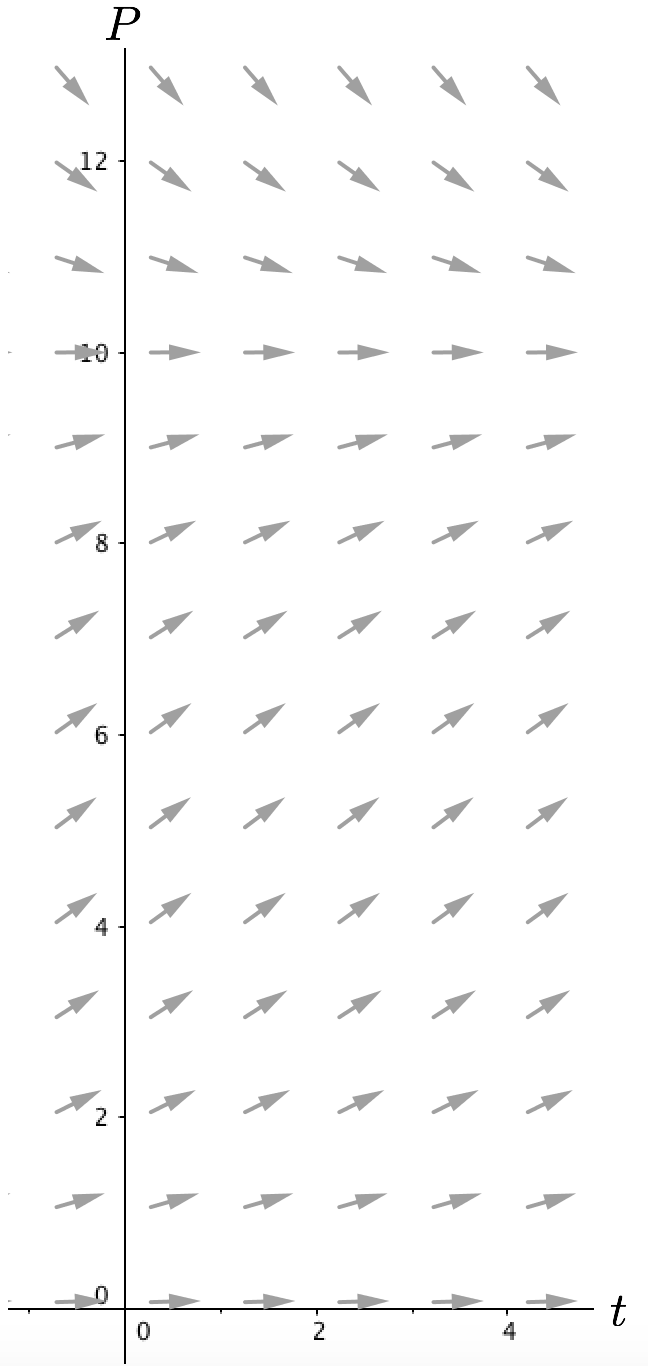
\includegraphics[width=2in]{03/03SlopeFieldFish.png}
\end{center}
 
\begin{enumerate}[resume]
\item \label{03problem2}
\begin{enumerate}
\item On the slope field above, stitch together in a tip to tail manner several tangent vectors to produce a graph of the population versus time if at time $t = 0$ we know there are 8 fish in the lake (again, think of 8 as scaled for say, 8000 or 80,000). \label{03problem3parta}
\vs
\item Reproduce your technique as much as possible using the Slope Field Stitcher applet, \\ \href{https://ggbm.at/FZn4WHeU}{\underline{https://ggbm.at/FZn4WHeU}}.  You can use the arrow buttons to move the initial vector around, and then create subsequent vectors to stitch on using the appropriate button. \label{03problem3partb}

\vspace{-.3in}\hspace{-0.75in}
\includegraphics[width=0.5in]{03/03SlopeFieldStitcherQR.png}
\end{enumerate}

\item	Explain how you are thinking about rate of change \textbf{in your method}. For example, is the rate of change constant over some increment? If yes, over what increment? If no, is the rate of change always changing? \label{03problem4}
\vfill

\clearpage

\item Using the differential equation $\displaystyle\frac{dP}{dt}=P\left(1-\frac{P}{20}\right)$ and initial condition $P(0) = 10$, Jos{\'e} and Julie started the following table to numerically keep track of their tip-to-tail method for connecting tangent vectors. Explain Jos{\'e}'s and Julie's approach and complete their table. \textbf{Round to two decimal places.} \label{03problem5}

{
\renewcommand{\arraystretch}{1.5}
\newcolumntype{R}{>{\centering\arraybackslash}X}%
\begin{tabularx}{.4\textwidth}{ |R|R|R| }
\hline
$t$ & $P$ & $\frac{dP}{dt}$\\\hline
0 & 10 & 5\\\hline
0.5 & 12.5 & \\\hline
1.0&&\\\hline
1.5&&\\\hline
\end{tabularx}}
\vfill

\item	Using the same differential equation and initial condition as Jos{\'e} and Julie, Derrick and Delores started their table as shown below. Explain how Derrick and Delores' approach is different from Jos{\'e} and Julie's and then complete their table. \textbf{Round to two decimal places.} \label{03problem6}

{
$\displaystyle  \frac{dP}{dt}=P\left( 1-\frac{P}{20}\right) $
 
\renewcommand{\arraystretch}{1.5}
\newcolumntype{R}{>{\centering\arraybackslash}X}%
\begin{tabularx}{.4\textwidth}{ |R|R|R| }
\hline
$t$ & $P$ & $\frac{dP}{dt}$\\\hline
0 & 10 & 5\\\hline
.25 & 11.25 & \\\hline
.5&&\\\hline
.75&&\\\hline
\end{tabularx}}
\vfill

\item Which approach do you think is more accurate and why? \label{03problem7}
\vfill

\clearpage

\item
\begin{enumerate}
\item Consider the differential equation $\displaystyle\frac{dy}{dt}=y+t$ and initial condition $y(0) = 4$. Use Jos{\'e} and Julie's approach to find $y(1.5)$. Show your work graphically and in a table of values. \label{03problem8parta}
\vfill
\vfill
\item Is your value for $y(1.5)$ the exact value or an approximate value? Explain. \label{03problem8partb}
\vfill
\end{enumerate}
\item	\textbf{Generalizing your tip-to-tail approach}. Create an equation-based procedure/algorithm that would allow you to predict future $y$-values for any differential equation $\displaystyle\frac{dy}{dt}$, any given initial condition, and any time increment. \label{03problem9} \vfill \vfill

\end{enumerate}

\clearpage
%%%%%%%%%%%%%%%%%%%%%%%%%%%%%%%%%%%%%%%%%%%%%%
\pagebegin{Homework Set 2}
 \begin{enumerate}

\item A slope field for the differential equation $\displaystyle\frac{dy}{dt}=0.5(y+t)$ is shown below. \label{03HWproblem1}
\begin{center}
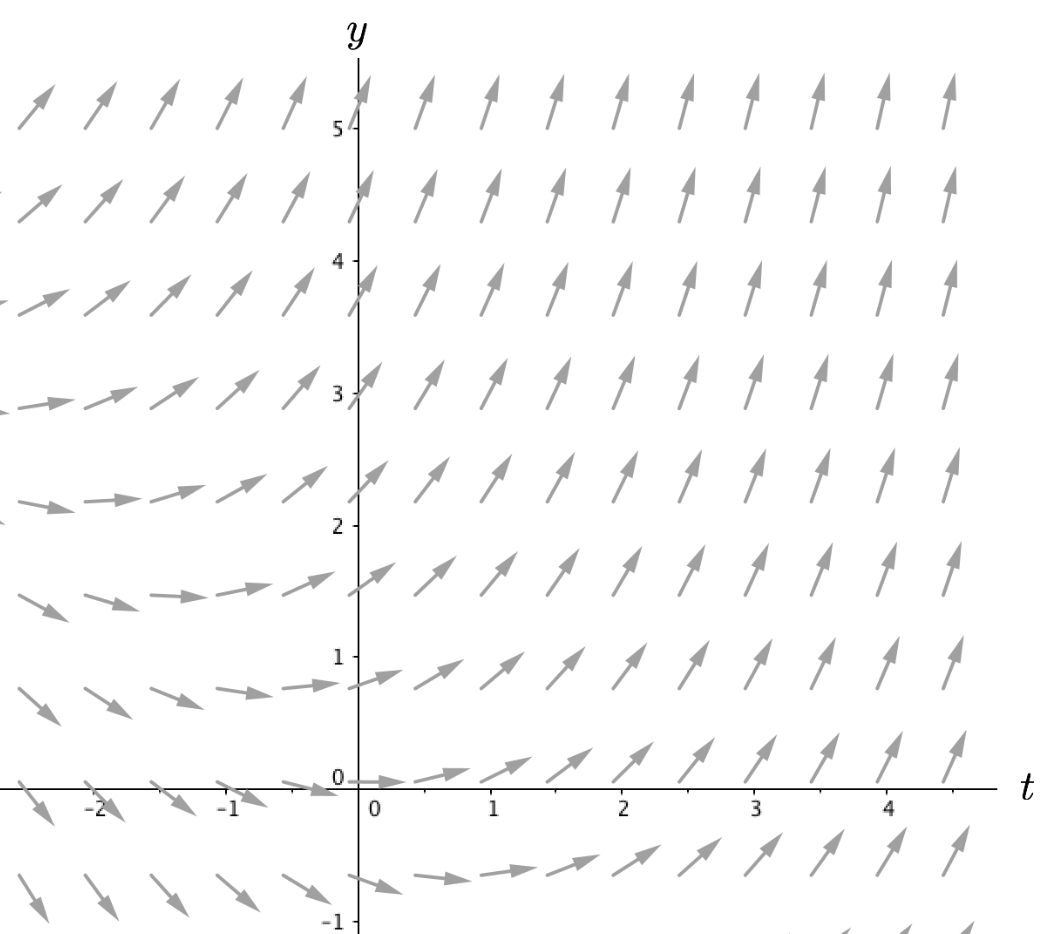
\includegraphics[width=6in]{03/03HWSlopeField1.png}
\end{center}
\begin{enumerate}
\item	For the initial condition of $y(0) = 1$, sketch on the above slope field what you think two iterations of the ``tip-to-tail'' method with a step size of 1 unit should look like. Do this \textbf{without} doing any computations. \label{03HWproblem1parta}
\item	Again, without doing any computations, sketch on the same slope field what you think three iterations with a step size of 0.5 units should look like for the same initial condition (perhaps using a different color). \label{03HWproblem1partb}
\item	Use the tip-to-tail ({\em i.e.}, Euler's) method to numerically compute approximations for parts \ref{03HWproblem1parta} and \ref{03HWproblem1partb} and then compare your graphical predictions to the numerical results. \label{03HWproblem1partc}
\end{enumerate}

\begin{comment}
\begin{hwsoln}
\begin{enumerate}
\item See picture.
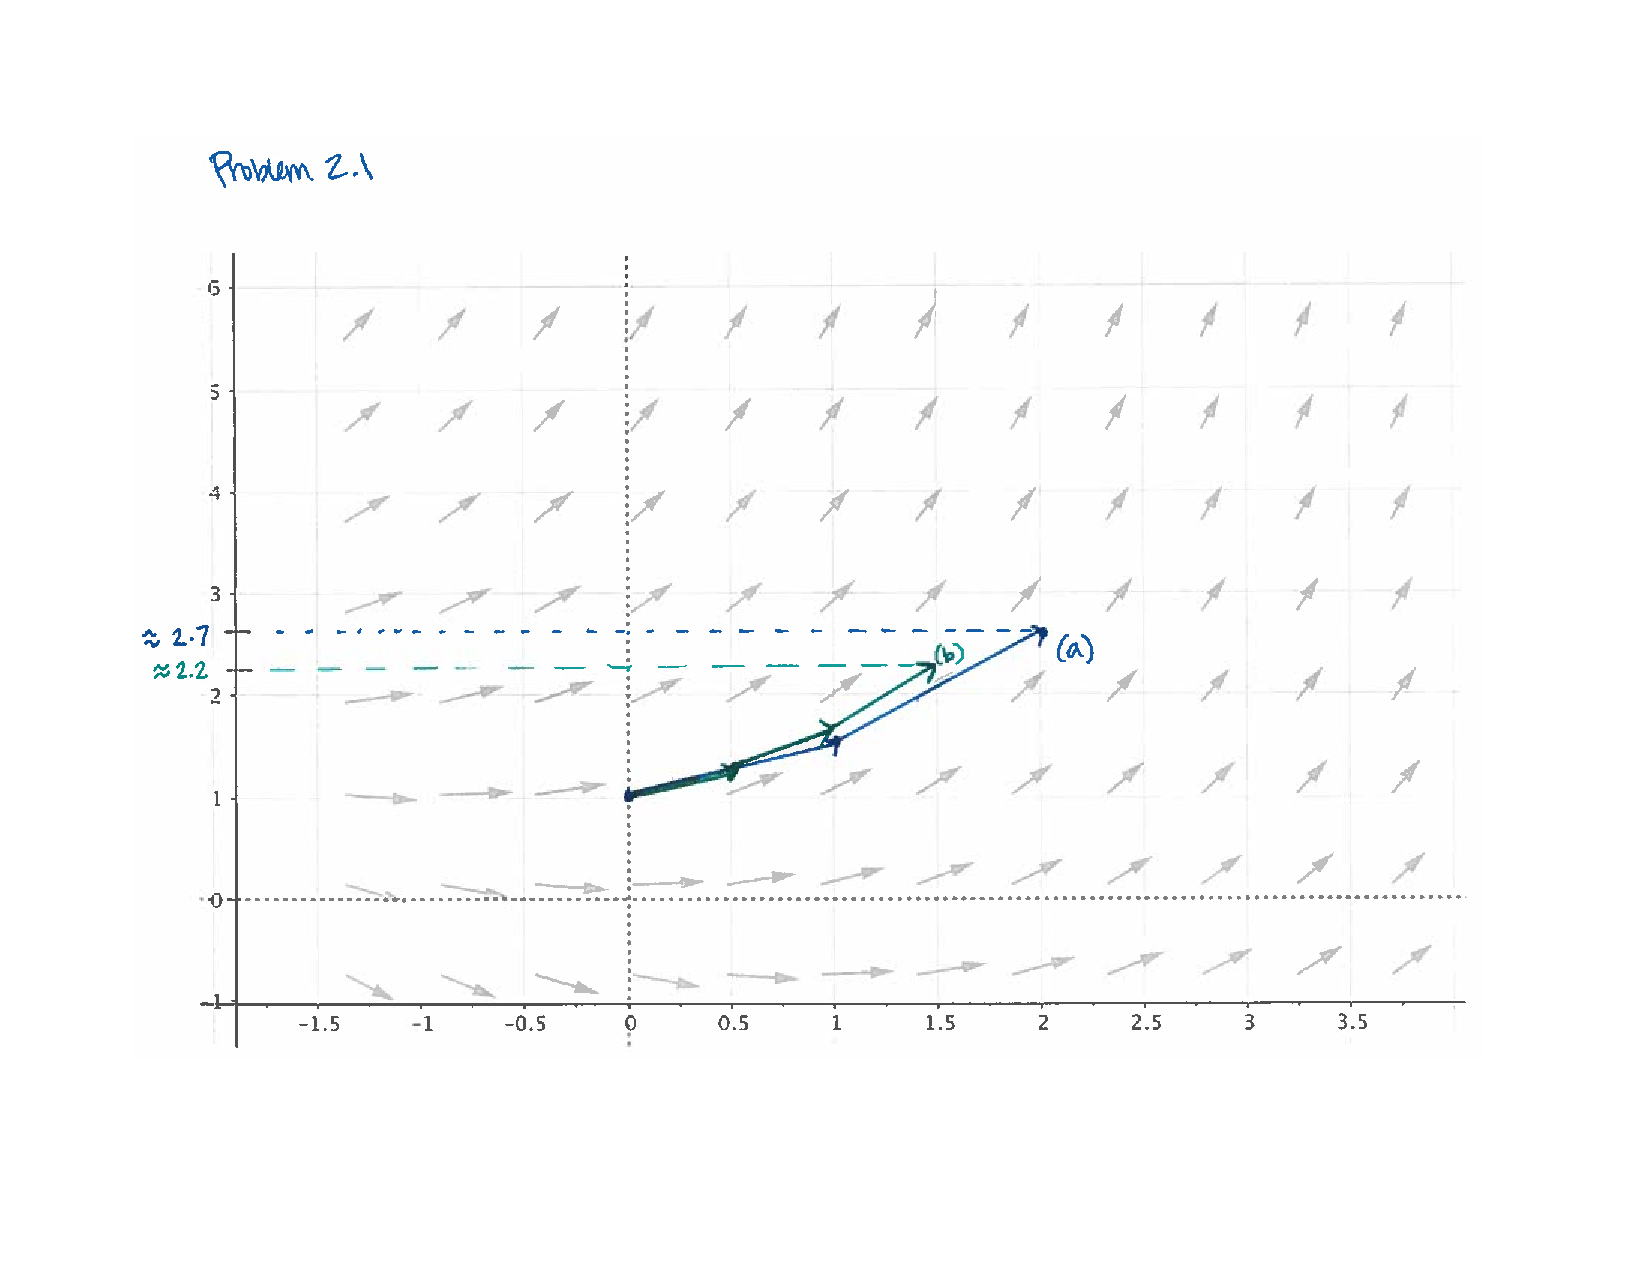
\includegraphics[width=4in]{03/03StitchOnMesoln.pdf}
\item See picture.
\item Given the initial condition $y(0) = 1$ and $\Delta t=1$, two steps of Euler's method gives the following:

$\frac{dy}{dt}\Big|_{t=0} = 0.5 (1+0) = \frac{1}{2} \quad \implies y(1)\approx y(0)+\frac{1}{2} = \frac{3}{2}  \\
\frac{dy}{dt}\Big|_{t=1} = 0.5 \left(\frac{3}{2}+1\right) = \left(\frac{1}{2}\right)\left(\frac{5}{2}\right) = \frac{5}{4} \quad \implies y(2)\approx y(1)+\frac{5}{4} = \frac{11}{4} = 2.75\\\textrm{(pretty close to the picture!)}$
\vs
Now using three iterations of Euler's method with $\Delta t=\frac{1}{2}$ we have:\\
$ \frac{dy}{dt}\Big|_{t=0} = 0.5 (1+0) = \frac{1}{2} \quad \implies y\left(\frac{1}{2}\right)\approx y(0)+\left(\frac{1}{2}\right)\left(\frac{1}{2}\right) = \frac{5}{4}  \\
\frac{dy}{dt}\Big|_{t=0.5} = 0.5 \left(\frac{5}{4}+\frac{1}{2}\right)  = \frac{7}{8} \quad \implies y(1)\approx y\left(\frac{1}{2}\right)+\frac{1}{2}\left(\frac{7}{8}\right)= \frac{5}{4}+\frac{7}{16} = \frac{27}{16}\\
\frac{dy}{dt}\Big|_{t=1} = 0.5 \left(\frac{27}{16}+1\right)  = \frac{43}{32} \quad \implies y\left( \frac{3}{2} \right)\approx y(1)+\frac{1}{2}\left(\frac{43}{32}\right) = \frac{27}{16} +\frac{43}{64}= 2.36$\\
(again, pretty close to the picture!)

\end{enumerate}
\end{hwsoln}
\end{comment}

\clearpage

\item Consider a differential equation with the given slope field and the initial value $y(0)=1$. \label{03HWproblem2}
\begin{center}
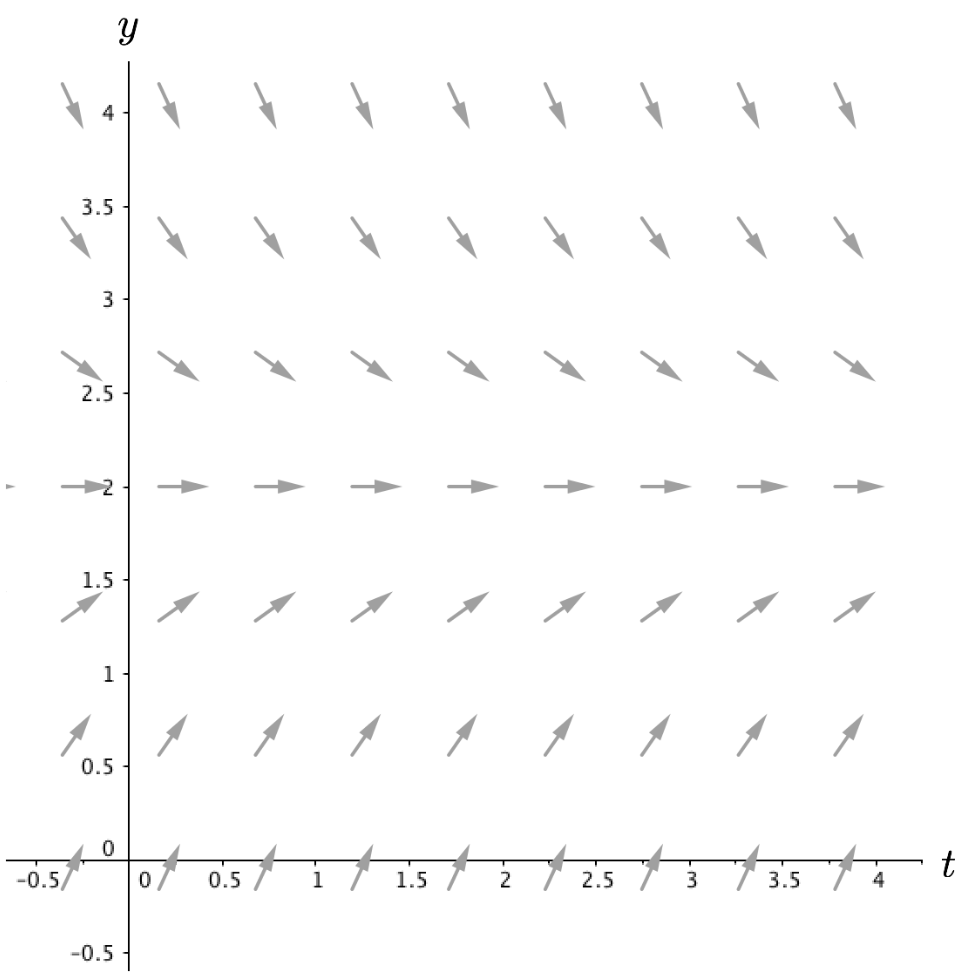
\includegraphics[width=5in]{03/03HWSlopeField2.png}
\end{center}
\begin{enumerate}
\item Explain why, if you wanted to approximate $y(2)$ using two steps of Euler's method, you would need $\Delta t = 1$.  \label{03HWproblem2parta}
\item Use a straight edge to graph two steps of Euler's method to approximate $y(2)$. \label{03HWproblem2partb}
\item This time, instead of using two steps of Euler's method, sketch on the same slope field what it would look like if you used four steps of Euler's method to approximate $y(2)$. \label{03HWproblem2partc}
\item Besides the obvious difference that the step size is different, state two other things that are different between your answers to parts \ref{03HWproblem2partb} and \ref{03HWproblem2partc}. \label{03HWproblem2partd}
\item Besides the obvious fact that they both use Euler's method, what is similar about the first step to your answers to parts \ref{03HWproblem2partb} and \ref{03HWproblem2partc}? \label{03HWproblem2parte}

\end{enumerate}

\begin{comment}
\begin{hwsoln}
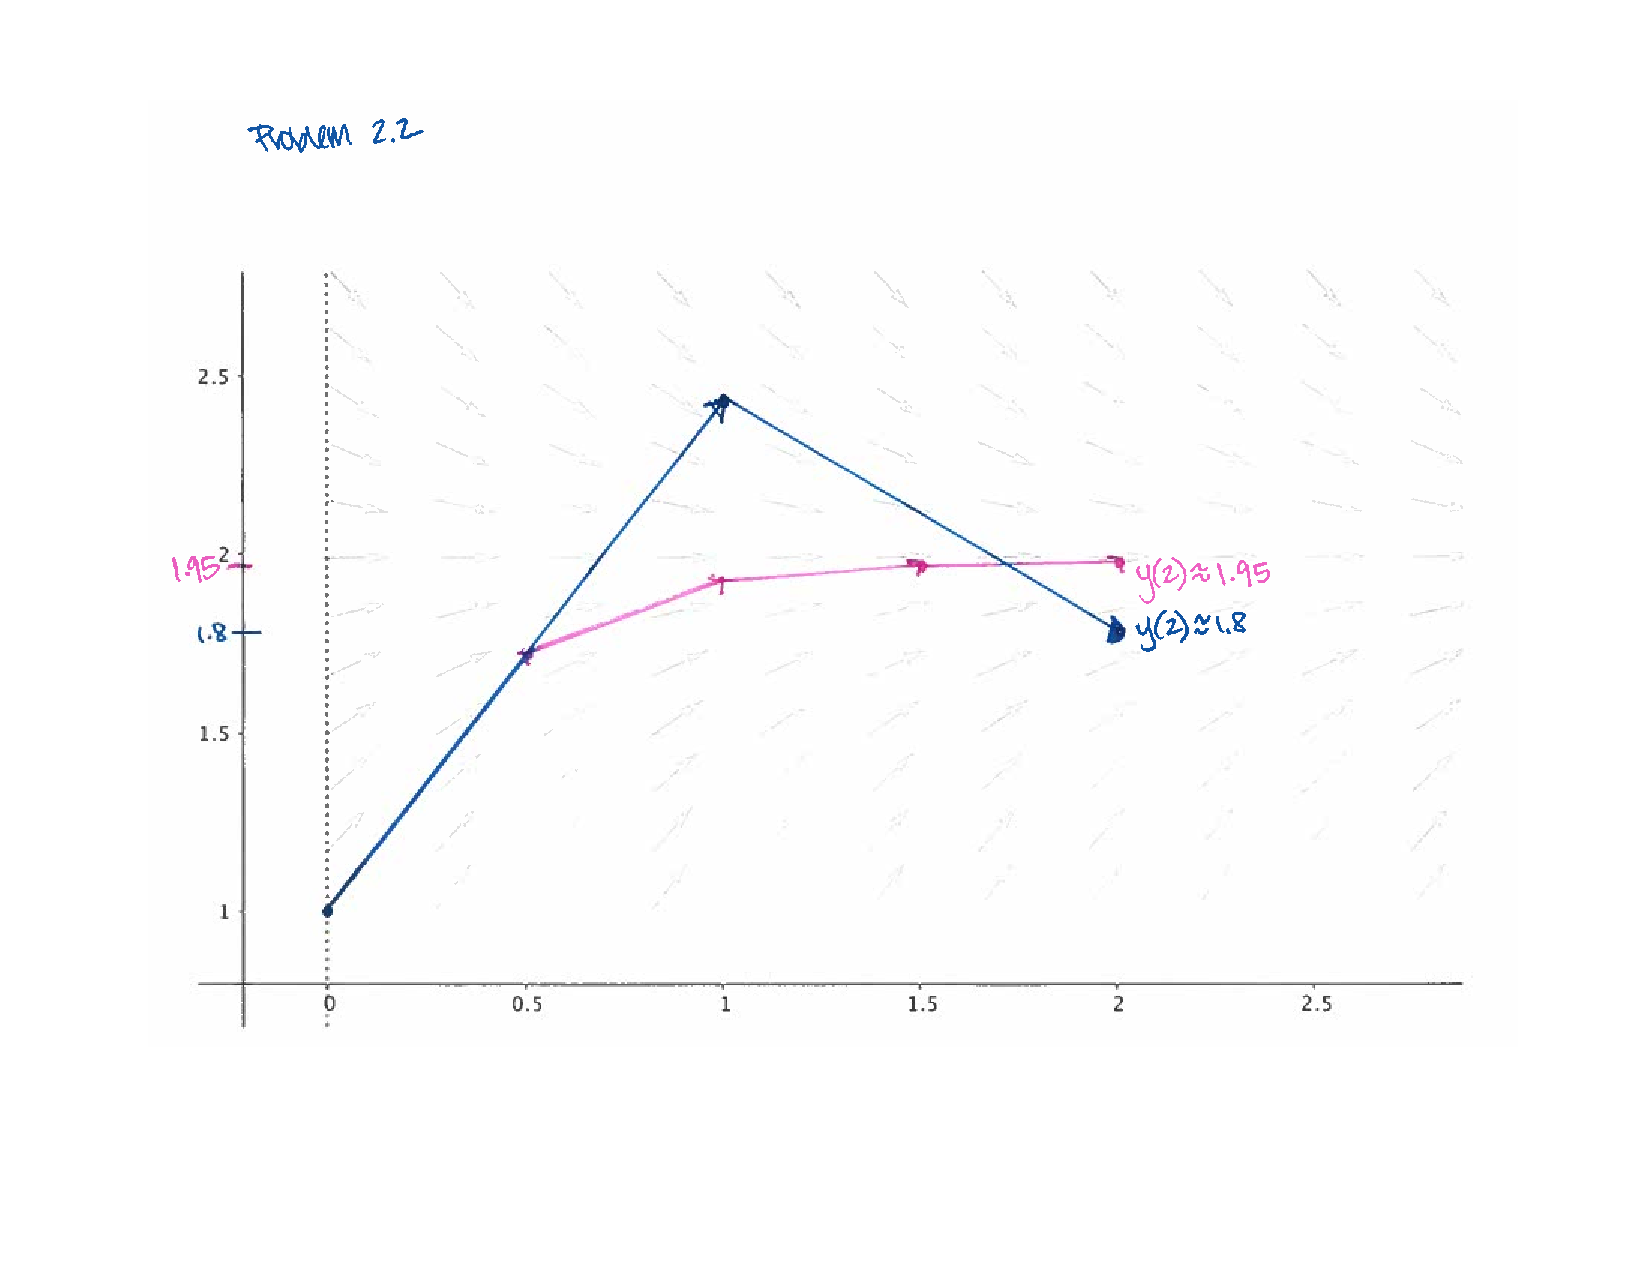
\includegraphics[width=4in]{03/03Eulergraphicalsoln}
\begin{enumerate}
\item See picture (blue).  $y(2)\approx 1.8$.
\item See picture (pink).  $y(2)\approx 1.95$.
\item The larger step size is almost certainly less accurate (or will be in most cases) because it assumes a constant slope for a longer period of time despite the actual solution having a constantly changing slope.  Plus, the larger step size ends up using approximate $y$-values on either side of the constant solution $y=2$, and crosses over this line during Euler's method, which wouldn't be true of an exact solution curve.  The smaller step size solution here ``looks'' more like what we'd expect of an exact solution. {\em (Keep in mind the students still don't know about Uniqueness, officially, so it's okay if this reasoning is a bit vague or incomplete.)}
\item These solutions are similar in the fact that they're both just approximations, and they both end up producing approximate $y$-values less than 2.
\end{enumerate}
\end{hwsoln}
\end{comment}

\clearpage

\item	Suppose we have a rate of change equation and initial condition for the population of raccoons in Lake County. Below is a graph of an \textbf{exact} solution. \label{03HWproblem3}

\begin{center}
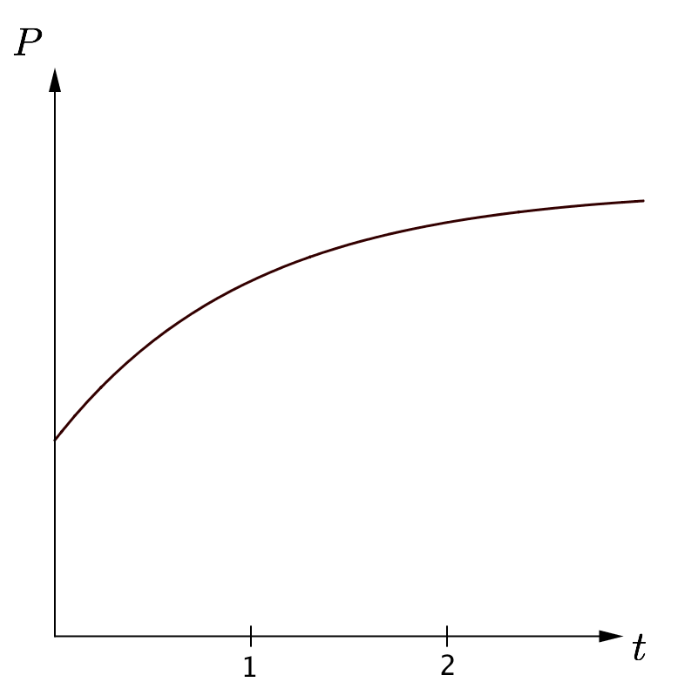
\includegraphics[width=2in]{03/03HWLotRExact.png}
\end{center}

Merry, Pippin, and Sam attempted to use the ``tip-to-tail'' Euler method to predict what the population of raccoons would be at time $t = 2$, with time increments one unit.  However, they arrived at different graphs for their predictions.  Their predictions are given below, and are shown with the exact solution.

\begin{tabular}{ccc}
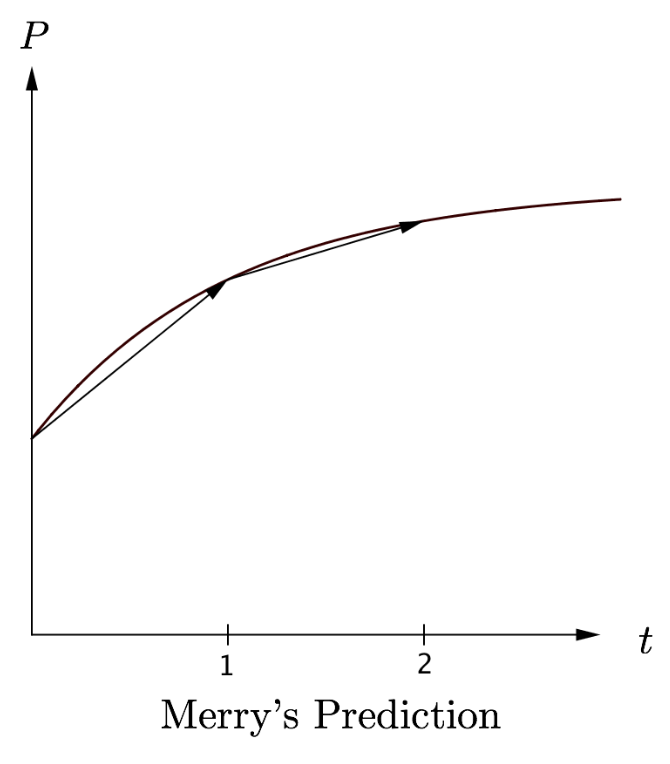
\includegraphics[width=2in]{03/03HWLotRMerry.png} & 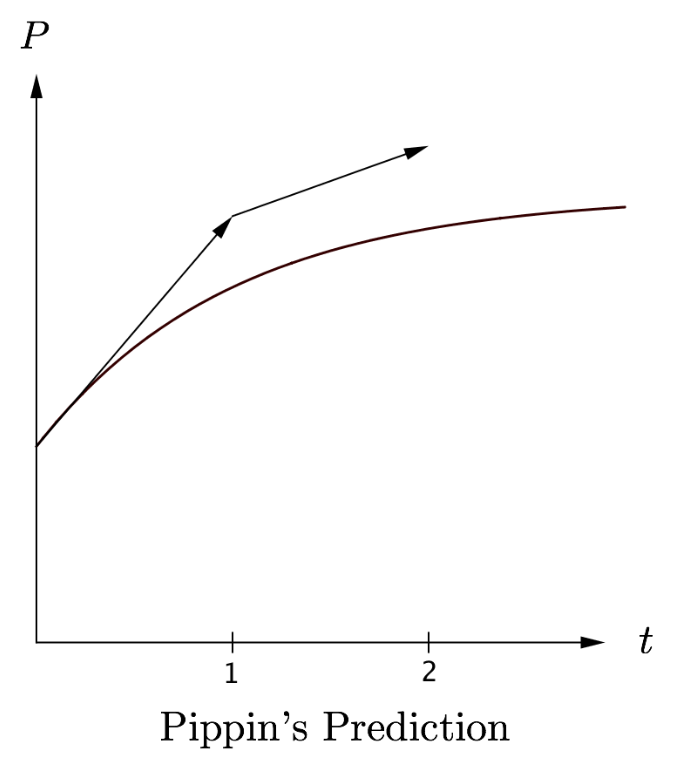
\includegraphics[width=2in]{03/03HWLotRPippin.png} & 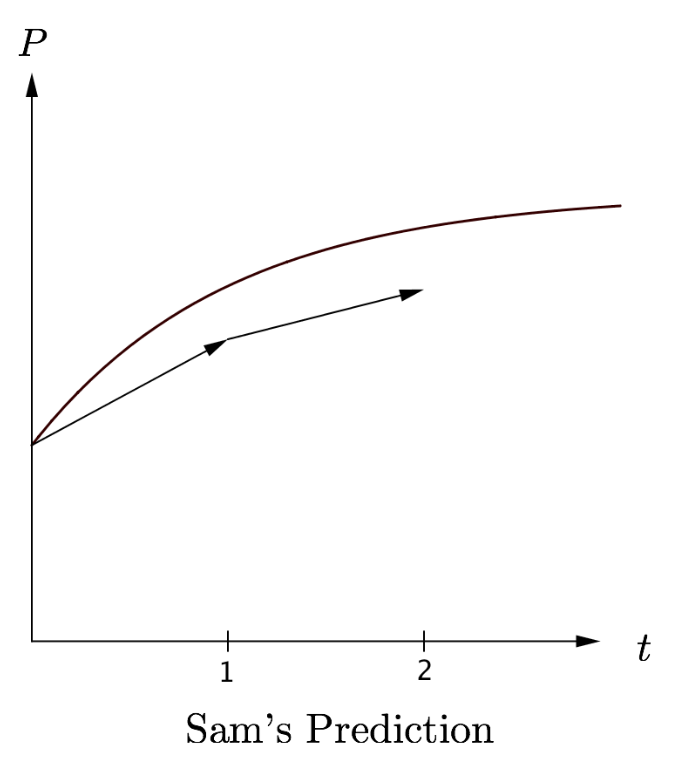
\includegraphics[width=2in]{03/03HWLotRSam.png}\\
\end{tabular}

For each prediction, give reasons as to whether or not each person illustrated the correct relationship between Euler's method and the exact solution. 

\item Suppose the function $y(t) = 6t +1$ is a solution to a particular differential equation. For the initial condition $y(0) = 1$, is a graph of the tip-to-tail Euler method exactly the same as the graph of the exact solution? Does your response depend on step size? Explain. \label{03HWproblem4}

\begin{comment}
\begin{hwsoln}
In this case, since $y(t)= 6t +1$ is a \textsl{linear} solution, if we plot a slope vector (in the $(t,y)$-plane) with initial condition $y(0) = 1$ it has to have the same slope as our exact solution  (because our solution has to satisfy the differential equation, which determines slope at every point!).  Thus, our slope vector at $y(0) = 1$ lies on the line $y(t)= 6t +1$.  This is true regardless how long we make it, thus the tip-to-tail Euler method will give us something on this line no matter what our step size is.  Therefore, Euler's method gives you approximations that are exact in this case, because they all lie on the same straight line solution.
\end{hwsoln}
\end{comment}

\item Compute by hand four steps of the tip-to-tail Euler method for the differential equation $\displaystyle\frac{dy}{dt}=y-t$  with initial condition $y(0) = 2$ and step size 0.5. \label{03HWproblem5}

\begin{comment}
\begin{hwsoln}
(Check that some calculations are shown.)  \\Using $y(0) = 2$ and  four steps with $\Delta t=0.5$ yields $y(2)\approx 8.0625$.
\end{hwsoln}
\end{comment}

\clearpage

\item	\textbf{Euler's Method Using a Spreadsheet.} Learning to use a spread sheet for various applications in engineering and mathematics is a valuable skill. Your task in this problem is to use Excel to generate as many steps of the Euler method that you want. \textit{If you are already familiar with Excel, skip the example below and go directly to part a}. \label{03HWproblem6}

EXAMPLE:  Here are step by step instructions for how to use Excel to generate 15 steps of the algorithm   $Y_{\textrm{next}} = 2 \cdot Y_{\textrm{now}} + 1$ with initial condition $Y = 3$. 

\begin{itemize}
\item	Open an Excel workbook 
\item	Select cell A1 by clicking on the cell in this location and type in Ynow as a column heading
\item	Select cell B1 and create a column heading called Ynext
\item	Select cell A2 and type in the number 3 (this is the given initial Y-value)
\item	Select cell B2 and type =2*A2+1 (after pressing Enter the number 7 will appear in this cell)
\item	Select cell A3 and type =B2
\item	Select and copy cell B2  (An animated dashed-line will appear around the cell)
\item	Select cells B3 through B15 and paste 
\item	Select and copy cell A3
\item	Select cells A4 through A15 and paste
\item	Do a few hand computations to verify the results

\end{itemize}
\begin{enumerate}
\item	Using a step size $\Delta t$ of your choice, figure out how to use Excel to generate at least 20 steps for Euler's method, $\displaystyle y_{\textrm{next}} = y_{\textrm{now}} + (\frac{dy}{dt})_{now}\cdot\Delta t$, for the differential equation $\displaystyle\frac{dy}{dt}=0.3y(1-\frac{y}{12.5})$ with initial condition $y(0) = 3$. In order to make it easier to graph the results, make your first column $t_{\textrm{now}}$ and your second column $y_{\textrm{now}}$. Turn in a print out your results and verify the first three steps by hand. \label{03HWproblem6parta}

\item	Use the Chart Wizard scatter plot option to create a graph of your $(t, y)$ data from part \ref{03HWproblem6parta}. An easy way to do this is to first highlight all the data in the $t_{\textrm{now}}$ and $y_{\textrm{now}}$ columns, select Chart Wizard, and follow the prompts. Turn in a print out of your results. \label{03HWproblem6partb}
\end{enumerate}

\begin{comment}
\begin{hwsoln}
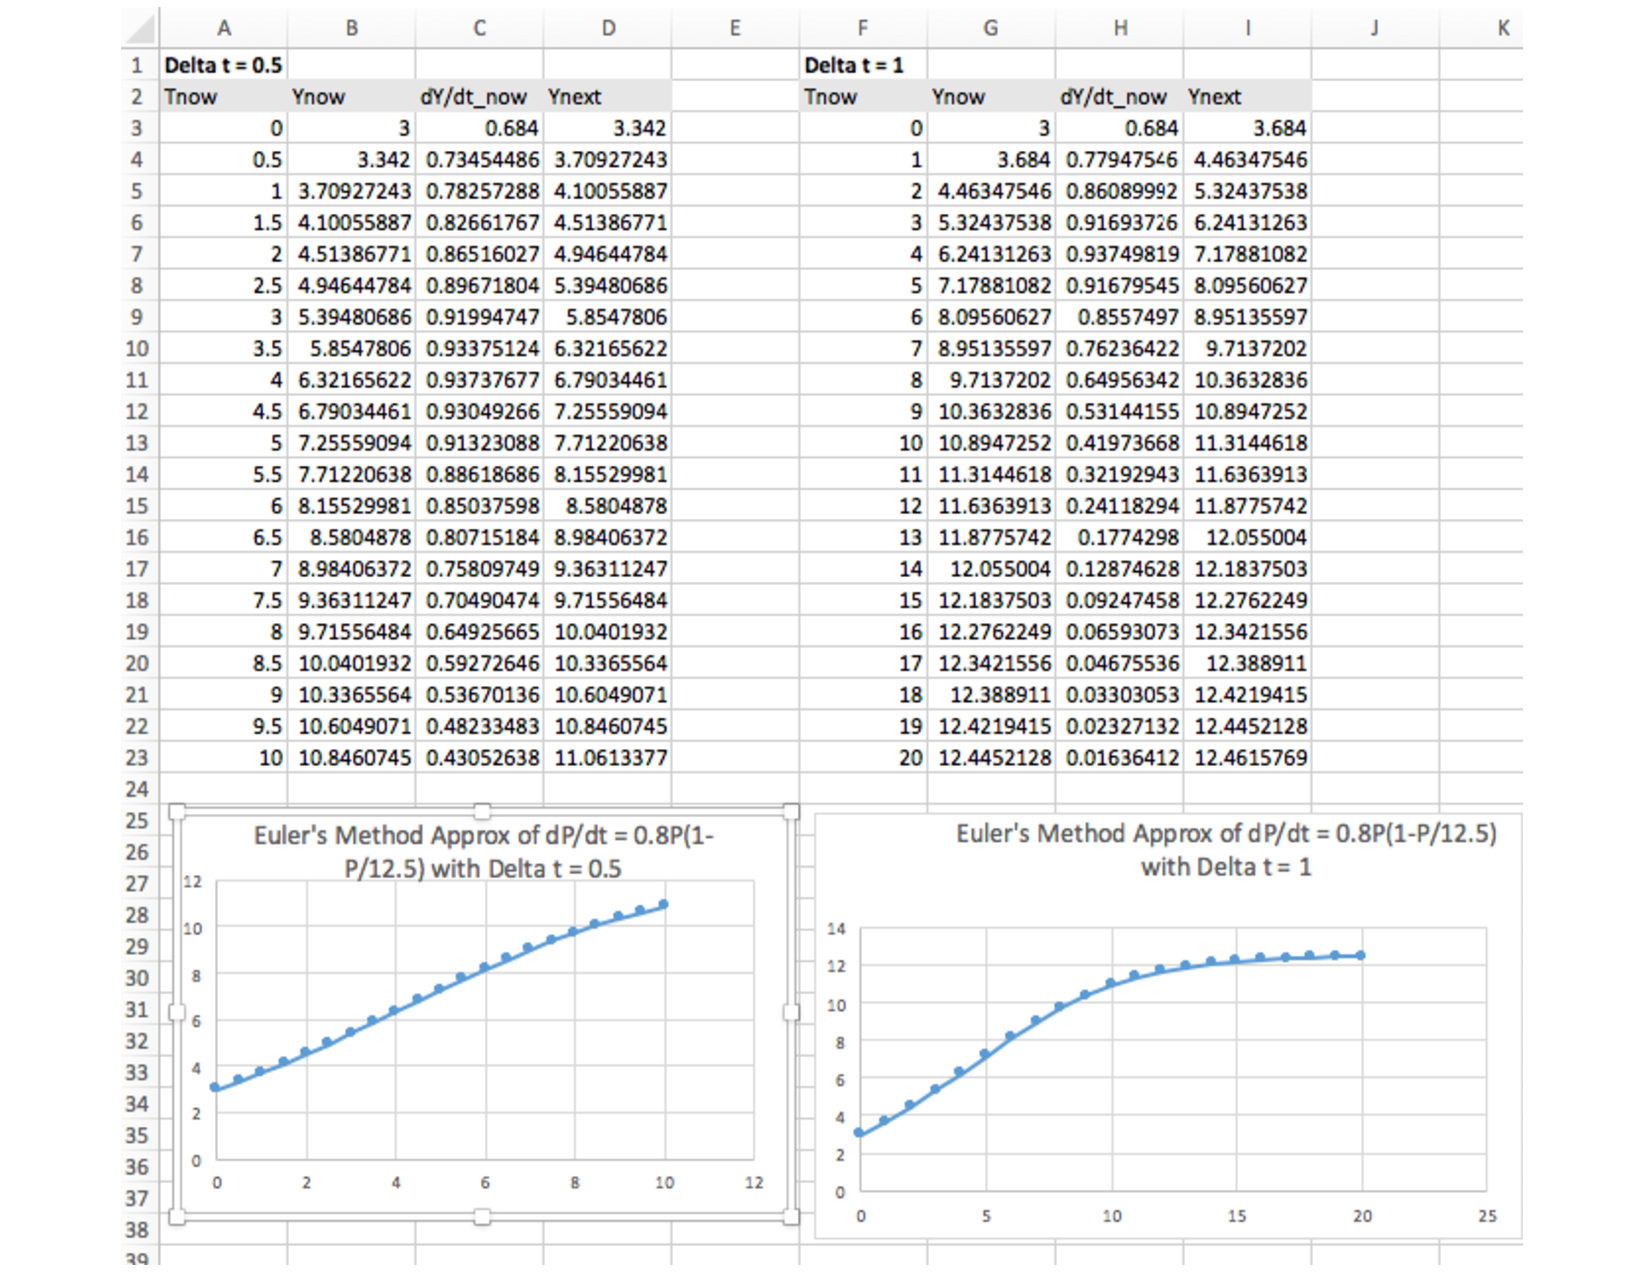
\includegraphics[width=5in]{03/03Eulerexcel.pdf}
\end{hwsoln}
\end{comment}

\item	Two students are having a discussion about the equal sign in the rate of change equation $\displaystyle\frac{dP}{dt} = 0.5P\left(1 - \frac{P}{100}\right)$. One student says he thinks about the equal sign as instructions for calculating. The other student says he thinks about the equal sign as a kind of mirror. How do you think about the equal sign in a rate of change equation? \label{03HWproblem7}

\clearpage

\item A group of scientists created the differential equation $\displaystyle\frac{dP}{dt}=0.8P\left(1-\frac{P}{5}\right)$  to predict future fish populations in Lake Minnetonka, where $P$ represents thousands of fish and $t$ is in years. \label{03HWproblem8}

\begin{enumerate}
\item	If you were to plot a slope field for this rate of change equation, what window for the $P$ and $t$ values would you use to make sure the most important features are clearly shown? Explain. \label{03HWproblem8parta}
\item	What does this rate of change equation predict about the long-term outcome of the fish population if the initial population is 2 ({\em i.e.}, $P = 2$ at $t = 0$)? How about if $P = 6$ at $t = 0$? \label{03HWproblem8partb}
\item	Why are the predictions you made in part \ref{03HWproblem8partb} reasonable (or not) for a fish population? Explain. \label{03HWproblem8partc}
\item	Carry out by hand three steps of Euler's method with a step size of 0.5 for the initial condition $P(0) = 5$. \label{03HWproblem8partd}
\end{enumerate}

\end{enumerate}
